
\section{Graph-theoretic connections available by 1981}
\label{sec:graphs}

The arithmetic equivalence classes admit a direct interpretation in terms of
flows and incidence operators on a countable directed graph.  This description
is useful in three ways: it explains Euler-factor cancellation, gives a
quantitative stability bound, and supplies finite graph models of the
literal summation operators.

\subsection{The prime path and its incidence boundary}

Let \(G_P\) be the directed ray with vertices \(v_j=p_j\) and edges
\(b_j:p_j\to p_{j+1}\), \(j\ge1\).  For an endpoint perturbation
\(a_j=p_{j+e_j}\), put the binary flow \(e_j\in\{0,1\}\) on \(b_j\).
We use the incidence convention
\[
 (\partial e)_j=e_j-e_{j-1},\qquad e_0=0,
\]
so an occupied edge contributes \(+1\) at its source and \(-1\) at its
target.  This is the (signed) vertex boundary of the edge flow.

\begin{center}
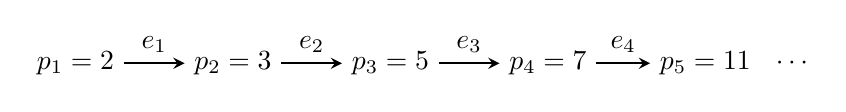
\begin{tikzpicture}[>=stealth,baseline]
\node (a) at (0,0) {$p_1=2$};
\node (b) at (2,0) {$p_2=3$};
\node (c) at (4,0) {$p_3=5$};
\node (d) at (6,0) {$p_4=7$};
\node (e) at (8,0) {$p_5=11$};
\draw[->,thick] (a)--node[above]{$e_1$}(b);
\draw[->,thick] (b)--node[above]{$e_2$}(c);
\draw[->,thick] (c)--node[above]{$e_3$}(d);
\draw[->,thick] (d)--node[above]{$e_4$}(e);
\node at (9.1,0) {$\cdots$};
\end{tikzpicture}
\end{center}

Put \(g_s(x)=\log(1-x^{-s})\), with the branch specified by its
convergent power series for \(x>1\) and \(\Re s>0\).
An elementary discrete-Stokes formula is
\begin{equation}\label{eq:graph-stokes}
 \sum_{n=1}^{N}e_n\bigl(g_s(p_n)-g_s(p_{n+1})\bigr)
 =\sum_{j=1}^{N}(\partial e)_j g_s(p_j)
       -e_Ng_s(p_{N+1}).
\end{equation}
The left side converges absolutely and locally uniformly for \(\Re s>0\).
Indeed, on a compact subset of that half-plane,
\[
 |g'_s(x)|\le C_K x^{-1-\sigma_K}\quad(x\ge2)
\]
for some \(\sigma_K>0\), and
\(\sum_n\int_{p_n}^{p_{n+1}}x^{-1-\sigma_K}\,dx<\infty\).
Since \(g_s(p_n)\to0\), taking \(N\to\infty\) in
\eqref{eq:graph-stokes} gives
\begin{equation}\label{eq:graph-product}
 \boxed{\quad
 \log Q_e(s)
 =\sum_{n\ge1}e_n\bigl[g_s(p_n)-g_s(p_{n+1})\bigr]
 =\sum_{j\ge1}(\partial e)_j g_s(p_j),\quad \Re s>0.
 \quad}
\end{equation}
The second series in \eqref{eq:graph-product} need not be absolutely
convergent: its equality follows from the boundary term in
\eqref{eq:graph-stokes}, not from arbitrary rearrangement.

For \(e_n=1\) on every edge, the interior boundary vanishes and
\(\partial e=(1,0,0,\ldots)\).  Therefore
\[
 \log Q_e(s)=g_s(2),\qquad Q_e(s)=1-2^{-s}.
\]
An infinite occupied ray has only a finite source boundary.  If instead
\(e_n=1\) precisely for \(u\le n\le v\), then
\[
 \partial e=\mathbf 1_{\{u\}}-\mathbf 1_{\{v+1\}},
 \qquad Q_e(s)=\frac{1-p_u^{-s}}{1-p_{v+1}^{-s}}.
\]
For alternating occupied edges, the graph boundary is supported at
every vertex, explaining why cancellation is much weaker.

\subsection{Weighted graph variation and quantitative conditioning}

For a bounded integer-valued edge flow \(h=(h_j)\), let
\begin{equation}\label{eq:graph-TV}
 V_\delta(h):=\sum_{j\ge1}p_j^{-\delta}
                  |h_j-h_{j-1}|,\qquad h_0=0,\quad\delta>0.
\end{equation}
This is the weighted \(\ell^1\)-norm of its incidence boundary,
a discrete bounded-variation quantity on \(G_P\).
For binary perturbations $e,f$, the weighted boundary sum is a sufficient
condition for bounded comparison. It measures transitions in an edge flow,
rather than merely counting moved primes.

\begin{proposition}[Graph-variation stability bound]
\label{prop:graph-conditioning}
Let \(e,f\) be endpoint perturbations and \(0<\delta\le1\).
If \(V_\delta(e-f)<\infty\), then
\(R_{e/f}=Q_e/Q_f\) and its inverse belong to
\(H^\infty(\Re s>\delta)\), and
\begin{equation}\label{eq:graph-stability}
 \max\{\|R_{e/f}\|_\infty,\|R_{e/f}^{-1}\|_\infty\}
 \le \exp\!\left(\frac{V_\delta(e-f)}{1-2^{-\delta}}\right).
\end{equation}
The product of the two operator-multiplier norm bounds is at most
\(\exp(2V_\delta(e-f)/(1-2^{-\delta}))\).
\end{proposition}
\begin{proof}
Put \(h=e-f\), and \(c_j=h_j-h_{j-1}\).
For \(\Re s>\delta\), the estimate
\[
 |\log(1-p_j^{-s})|
 \le \frac{p_j^{-\delta}}{1-p_j^{-\delta}}
 \le \frac{p_j^{-\delta}}{1-2^{-\delta}}
\]
shows that \(\sum_j c_jg_s(p_j)\) converges absolutely and uniformly
and has modulus at most
\(V_\delta(h)/(1-2^{-\delta})\).
Exponentiate \eqref{eq:graph-product} for the quotient, and then
apply the same argument with \(-h\).
\end{proof}

The additive group of bounded integer edge flows contains the subgroup
\(\{h:V_\delta(h)<\infty\}\).
Consequently the binary endpoint perturbations map to equivalence
classes in the quotient by this subgroup.  This is a convenient
graph-cochain description of the arithmetic classification; it does
\emph{not} assert ordinary graph-Laplacian spectral equivalence.

\subsection{A signed-frequency graph for arbitrary interior shifts}

The same bookkeeping works beyond the endpoints.  For a finite
perturbation \(A_N=(a_1,\ldots,a_N)\), draw the oriented edge
\(p_n\to a_n\) on the vertex set of all distinct frequencies
\(\{p_1,\ldots,p_N,a_1,\ldots,a_N\}\).  A loop contributes zero.
The signed vertex boundary is the atomic measure
\[
 \mu_{A,N}:=\sum_{n=1}^N(\delta_{p_n}-\delta_{a_n}).
\]
For every \(\Re s>0\), the finite Euler quotient satisfies
\begin{equation}\label{eq:graph-atomic}
 \log Q_{A,N}(s)=
 \int_{(1,\infty)}\log(1-x^{-s})\,d\mu_{A,N}(x).
\end{equation}
If two edges share a frequency endpoint, their incidence
coefficients may cancel.  Cancellation of this boundary is exact for shared endpoints. A complete
necessary condition for general interior shifts is not asserted.


\subsection{A bounded comparison on the original weighted Sobolev space}

The graph variation also controls the original dilation operators
without first passing to a Hardy-space multiplier representation.
Fix $S_k$ as in Section~\ref{sec:operators}, with
$\alpha=1/(2k)$, and write
$c_j=(e_j-f_j)-(e_{j-1}-f_{j-1})$.

\begin{theorem}[Norm-convergent graph-boundary comparison, new]
\label{thm:graph-Sk}
Suppose that
\begin{equation}\label{eq:graph-Sk-hyp}
 \sum_{j\ge1}|c_j|p_j^{-\alpha}<\infty.
\end{equation}
Then the product
\begin{equation}\label{eq:graph-Sk-operator}
 C_{e/f}=\prod_{j\ge1}(I-R_{p_j})^{c_j}
\end{equation}
converges in operator norm on $S_k$. It has a bounded inverse.
Moreover,
\begin{equation}\label{eq:graph-Sk-bound}
 \max\{\|C_{e/f}\|,\|C_{e/f}^{-1}\|\}
 \le \exp\left(
 \frac{\sum_{j\ge1}|c_j|p_j^{-\alpha}}
 {1-2^{-\alpha}}\right).
\end{equation}
On the algebraic domain $\mathcal D_k$, $C_{e/f}$ is the
multiplier with symbol $\zeta_{A_e}/\zeta_{A_f}$,
where the quotient is understood through its holomorphic
Euler-factor continuation.
\end{theorem}

\begin{proof}
A change of variables in each term of the $S_k$ norm gives
$\|R_p\|\le p^{-\alpha}$. Thus
$\|I-R_p\|\le1+p^{-\alpha}$ and
$\|(I-R_p)^{-1}\|\le(1-p^{-\alpha})^{-1}$.
The logarithms of both bounds are no larger than
$p^{-\alpha}/(1-p^{-\alpha})$.
The hypothesis ensures norm convergence of the products
with exponents $c_j$ and $-c_j$, and gives
\eqref{eq:graph-Sk-bound}. All the factors commute, so the
two products are inverses.
On $y^s$ the symbol is
$\prod_j(1-p_j^{-s})^{c_j}$.
The discrete-Stokes identity \eqref{eq:graph-stokes}
identifies that symbol with the ratio of the two
Euler-product comparisons. On logarithmic powers,
differentiate the normally convergent scalar identity.
\end{proof}

\begin{example}[A fully occupied prime path]
If every prime is moved to the next prime, then
$c_1=1$ and $c_j=0$ for $j>1$ (taking $f_j=0$).
Hence $C_{e/f}=I-R_2$. Infinite arithmetic
perturbations have collapsed to one boundedly invertible
operator factor.
\end{example}

\begin{remark}
This is a sufficient condition for bounded comparison.
It neither proves similarity by conjugation of the full
summation operators nor asserts anything about graph-Laplacian
isospectrality.
\end{remark}

\subsection{The multiplicative graph of generalized integers}

For \(A_N=(a_1,\ldots,a_N)\), consider the graded directed graph
\[
 \Gamma_{A_N}:\quad
 V=\mathbb Z_{\ge0}^{N},\qquad
 \nu\longrightarrow \nu+\mathbf e_j\quad(1\le j\le N).
\]
Give the vertex \(\nu\) the weight
\(w_s(\nu)=\prod_{j=1}^N a_j^{-s\nu_j}\).
Summing \emph{vertices}, rather than all directed paths, gives
\begin{equation}\label{eq:graph-vertexzeta}
 \sum_{\nu\in\mathbb Z_{\ge0}^N}w_s(\nu)
 =\prod_{j=1}^N(1-a_j^{-s})^{-1}
 =\zeta_{A,N}(s),\qquad\Re s>0.
\end{equation}
This vertex interpretation respects the multiplicities of
generalized integers.  For example, \(a_1=a_2=3\) produces
three exponent vectors of total degree two, all evaluating to \(9\);
accordingly the coefficient of \(3^{-2s}\) in
\((1-3^{-s})^{-2}\) is \(3\).  Counting directed paths instead
would introduce different, and incorrect, multiplicities.
The graph in \eqref{eq:graph-vertexzeta} is not an Ihara
nonbacktracking-cycle zeta construction.

\begin{proposition}[Convergent graph-transfer realization]
\label{prop:graph-transfer}
For \(\sigma>1\), let \(X_\sigma\) be the Banach space of functions
on \((0,1]\) with
\[
 \|f\|_{X_\sigma}:=\sup_{0<y\le1}y^{-\sigma}|f(y)|<\infty.
\]
Write \(D_a f(y)=f(y/a)\).  The operator products
\begin{equation}\label{eq:graph-resolvents}
 P_A=\prod_{n\ge1}(I-D_{a_n})^{-1},
 \qquad
 (I-qD_q)P_A\quad(q=2,3)
\end{equation}
converge in operator norm on \(X_\sigma\), and
\begin{equation}\label{eq:graph-literalsum}
 (I-qD_q)P_Af(y)
 =\sum_{m\in\mathcal N_A}
 \left[f(y/m)-qf(y/(qm))\right].
\end{equation}
All sums in \eqref{eq:graph-literalsum} converge absolutely in
\(X_\sigma\).  These operators are boundedly invertible on
\(X_\sigma\).
\end{proposition}
\begin{proof}
The dilation operators commute and
\(\|D_a\|_{X_\sigma}=a^{-\sigma}\).
Since \(a_n\ge p_n\) and
\(\sum_n p_n^{-\sigma}<\infty\), the two products
\(\prod_n(I-D_{a_n})^{-1}\) and
\(\prod_n(I-D_{a_n})\) converge in operator norm and
are inverses.  Expand each geometric series and pass to the
norm limit to obtain the generalized-integer sum with
multiplicity.  Finally,
\(\|qD_q\|=q^{1-\sigma}<1\), so \(I-qD_q\) is invertible
by a Neumann series.
\end{proof}

\begin{remark}[Scope of the graph model]
The space \(X_\sigma\), \(\sigma>1\), is the domain of an
\emph{absolutely convergent} graph-transfer representation.  It
does not contain the zeta-zero eigenfunctions \(y^\rho\) from the
critical strip and is not a substitute for the analytically
continued \(S_k\) operators.  In particular, Proposition
\ref{prop:graph-transfer} proves no kernel invariance in the
critical strip.  It supplies a natural discrete approximation
and separates the convergent graph mechanics from the deeper
operator-domain problem.
\end{remark}

\paragraph{Further graph questions.}
One can ask whether (i) weighted incidence-boundary classes
admit computable finite-section approximations with certified
tails; (ii) equality of closed graph-transfer domains forces
bounded comparison in a natural completion; and (iii) the
graph boundary at infinity controls comparison-operator
conditioning.  These are proposed investigations, not claims
about the spectrum of a graph Laplacian.
